\themaG
\graphicspath{{../Ch19_Les_triangles/Images/}}

\chapter{Les triangles}
\label{C09}


%%%%%%%%%%%%%%%%%%%%%%%%%%%%%%%%
%%%%%%%%%%%%%%%%%%%%%%%%%%%%%%%%
\begin{prerequis}[Connaissances et compétences abordées]
   \begin{itemize}
      \item Reconnaître, nommer, décrire des triangles, dont les triangles particuliers (triangle rectangle, triangle isocèle, triangle équilatéral).
      \item Vocabulaire associé à ces objets et à leurs propriétés : côté, sommet, angle, hauteur.
   \end{itemize}
\end{prerequis}

\vfill

\begin{debat}[Débat : vocabulaire du triangle] 
   Le mot {\bf triangle} est construit à partir du préfixe \og tri \fg, trois et angle, c'est donc un polygone à trois\dots{} angles ! À la renaissance, on hésite entre triangle et trigone (du grec trigônum). Les mathématiciens choisissent {\it triangle} et les astrologues {\it trigone}, qui donnera le mot {\it trigonométrie}, branche des mathématiques qui traite des relations entre distances et angles dans les triangles.
   \begin{center}
      \begin{pspicture}(0,-0.5)(4.3,4.2)
         \pspolygon[fillstyle=solid,fillcolor=A2](0,1.6)(4,0)(4.2,3.8)
         \rput[r](-0.3,1.6){Floride}
         \rput[l](4.4,4){Bermudes}
         \rput[l](4.3,0){Porto Rico}
      \end{pspicture}
   \end{center}
   \begin{cadre}[B2][F4]
      \begin{center}
         Vidéo : \href{https://www.youtube.com/watch?v=MUr7dgn8wdo}{\bf Le triangle des Bermudes}, chaîne YouTube {\it SYMPA}.
      \end{center}
   \end{cadre}
\end{debat}

\vfill

\textcolor{PartieGeometrie}{\large\sffamily\bfseries Cahier de compétences} : chapitre 10, exercices 1 à 5. 


%%%%%%%%%%%%%%%%%%%%%%%%%%%%%%%%%%%%
%%%%%%%%%%%%%%%%%%%%%%%%%%%%%%%%%%%%%
\activites

\begin{activite}[Avec des allumettes]
   {\bf Objectifs} : construire puis nommer des triangles. 
   \begin{QCM}
      Devant vous, vous avez douze allumettes. Pour chacune des questions suivantes, faire la construction si elle est possible avec des allumettes puis faire un dessin pour schématiser la situation. \\
      \begin{enumerate}
         \item Aligner cinq allumettes en les plaçant les unes à côté des autres.
         \smallskip
         \begin{center}
            \includegraphics[width=2.5cm]{allumette}\includegraphics[width=2.5cm]{/allumette}\includegraphics[width=2.5cm]{allumette}\includegraphics[width=2.5cm]{allumette}\includegraphics[width=2.5cm]{allumette}
         \end{center}
         \smallskip
         À partir de ce segment de longueur cinq allumettes et en utilisant les douze allumettes, combien peut-on construire de triangles différents ? Ces triangles sont-ils particuliers ? \\ [4cm]
         \item Mêmes questions si l'on place quatre allumettes côte à côte. \\ [3cm]
         \item Mêmes questions si l'on place six allumettes côte à côte. \\ [3cm]
         \item Mêmes questions si l'on place sept allumettes côte à côte ou plus. \\ [3cm]
      \end{enumerate}
   \end{QCM}
\end{activite}


%%%%%%%%%%%%%%%%%%%%%%%%%%%%%%%%
%%%%%%%%%%%%%%%%%%%%%%%%%%%%%%%%
\cours 

\section{Triangles particuliers} %%%%%%%%%

\begin{pspicture}(-5,-0.5)(10,2.5)
   \rput[l](-4,2){Triangle : }
   \rput[l](-4,1.5){$\bullet$ 3 angles}
   \rput[l](-4,1){$\bullet$ 3 côtés}
   \rput[l](-4,0.5){$\bullet$ 3 sommets}
   \rput[l](-4,0){$\bullet$ 3 hauteurs}
   \pstTriangle[PointSymbol=none,linecolor=A1](0,0){U}(4,0){I}(-1,2){O}
   \pstTriangle[PointSymbol=none,linecolor=A1](6,0){Y}(10,0){S}(7,2){E}
   \rput(2,2){\textcolor{A1}{côté}}
   \psline[linecolor=A1]{->}(1.5,1.8)(1.2,1.2)
   \rput(9,2){sommet}
   \psline{->}(8.2,2)(7.3,2)
   \pstMarkAngle[linecolor=J1,MarkAngleType=double,MarkAngleRadius=1,LabelSep=1.8]{O}{I}{U}{\textcolor{J1}{angle}}
   \psset{linecolor=B1}
   \psline(-1,0)(-1,2)
   \psline(-1,0.25)(-0.75,0.25)(-0.75,0)
   \psline(7,0)(7,2)
   \psframe(7,0)(7.25,0.25)
   \rput(5,1.5){\textcolor{B1}{hauteur}}
   \psline{->}(5.8,1.3)(6.8,1)
\end{pspicture}

\begin{definition}
   \begin{itemize}
      \item Un \textbf{triangle rectangle} est un triangle ayant un angle droit.
      \item Un \textbf{triangle isocèle} est un triangle ayant deux côtés de même longueur.
      \item Un triangle \textbf{équilatéral} est un triangle dont tous les côtés sont de même longueur.
   \end{itemize}
\end{definition}


{\psset{unit=0.9}
\begin{pspicture}(-2,-0.8)(4,2.8)
   \pstTriangle[PointSymbol=none](0,0){E}(4,0){C}(0,2){R}
   \pstRightAngle[linecolor=B1]{R}{E}{C}
   \rput(2,-0.5){triangle rectangle}
\end{pspicture}
\begin{pspicture}(-1.5,0.5)(5.5,3.3)
   \pstTriangle[PointSymbol=none](0,1){I}(4,1){O}(2,3){S}
   \pstSegmentMark[SegmentSymbol=MarkHashh,MarkAngle=90,linecolor=A1]{I}{S} 
   \pstSegmentMark[SegmentSymbol=MarkHashh,MarkAngle=90,linecolor=A1]{S}{O}
   \pstLineAB{I}{O}
   \pstMarkAngle[linecolor=J1,MarkAngleType=double]{S}{O}{I}{}
   \pstMarkAngle[linecolor=J1,MarkAngleType=double]{O}{I}{S}{}
   \rput(2,0.5){triangle isocèle}
\end{pspicture}
\begin{pspicture}(0,-0.5)(5,3.3)
   \pstTriangle[PointSymbol=none](0,0){E}(3,0){I}(1.5,2.55){Q}
   \psset{SegmentSymbol=MarkHash,MarkAngle=90,linecolor=A1}
   \pstSegmentMark{E}{Q} 
   \pstSegmentMark{I}{Q}
   \pstSegmentMark{I}{E}
   \psset{linecolor=A1}
   \pstMarkAngle[linecolor=J1]{Q}{I}{E}{}
   \pstMarkAngle[linecolor=J1]{I}{E}{Q}{}
   \pstMarkAngle[linecolor=J1]{E}{Q}{I}{}
   \rput(1.5,-0.5){triangle équilatéral}
\end{pspicture}}

\begin{remarques}
   un triangle équilatéral et un triangle isocèle particulier et un triangle rectangle peut être isocèle, mais pas équilatéral.
\end{remarques}


%%%%%%%%%%%%%%%%%%%%%%%%%%%%%%%%%%
\section{Construction d'un triangle connaissant trois longueurs}

\begin{methode*1}
   Pour construire un triangle $ABC$ dont on connaît les longueurs des trois côtés :
   \begin{itemize}
      \item on trace à la règle graduée l'un des côtés (en général le plus grand), par exemple $[AB]$ ;
      \item on trace un arc de cercle de centre $A$ et de rayon $AC$ ;
      \item on trace un arc de cercle de centre $B$ et de rayon $BC$ ;
      \item le point $C$ se situe à l'intersection des deux arcs de cercle.
   \end{itemize}
   \exercice
   Tracer le triangle $ABC$ tel que : $AB =\ucm{3,5}$ ; $BC =\ucm{2,2}$ et $CA =\ucm{3,2}$.
   %\correction
   \small
   \psset{unit=0.7}
   \begin{pspicture}(-1.5,-1.5)(4.8,3.5)
      \pstGeonode[PointSymbol=none,PosAngle={225,-45}](0,0){A}(3.5,0){B}
      \pstLineAB{A}{B}
      \rput(1.75,-0.25){3,5 cm}
   \end{pspicture}
   \begin{pspicture}(0,-1.5)(4.8,3.5)
      \pstGeonode[PointSymbol=none,PosAngle={225,-45}](0,0){A}(3.5,0){B}
      \pstLineAB{A}{B}
      \psset{linecolor=A1}
      \psarc(0,0){3.2}{30}{60}
      \rput{55}(0.8,1.3){\textcolor{A1}{3,2 cm}}
      \compas{1.5}{1.2}{55}{0.9}{34.5}
      \end{pspicture}
   \begin{pspicture}(0,-1.5)(4.8,3.5)
      \pstGeonode[PointSymbol=none,PosAngle={225,-45}](0,0){A}(3.5,0){B}
      \pstLineAB{A}{B}
      \psset{linecolor=A1}
      \psarc(0,0){3.2}{30}{60}
      \psset{linecolor=B1}
      \psarc[fillstyle=none](3.5,0){2.2}{90}{130}
      \rput{-45}(2.8,0.8){\textcolor{B1}{2,2 cm}}
      \compas{3.3}{1.1}{130}{0.9}{23}
   \end{pspicture}
   \begin{pspicture}(0,-1.5)(2,3.5)
      \pstGeonode[CurveType=polygon,PointSymbol=none,PosAngle={225,90,-45}](0,0){A}(2.5,2){C}(3.5,0){B}
   \end{pspicture}
\end{methode*1}

\begin{remarque}
   on a deux choix de construction pour $C$, d'un côté ou de l'autre du segment.
\end{remarque}


%%%%%%%%%%%%%%%%%%%%%%%%%%%%%%%%%%%
\exercicesbase

\begin{colonne*exercice}

\serie{Reconnaître des triangles} %%%%%%%%%%

\begin{exercice}
   Classer les triangles suivants dans le tableau.
   \begin{center}
      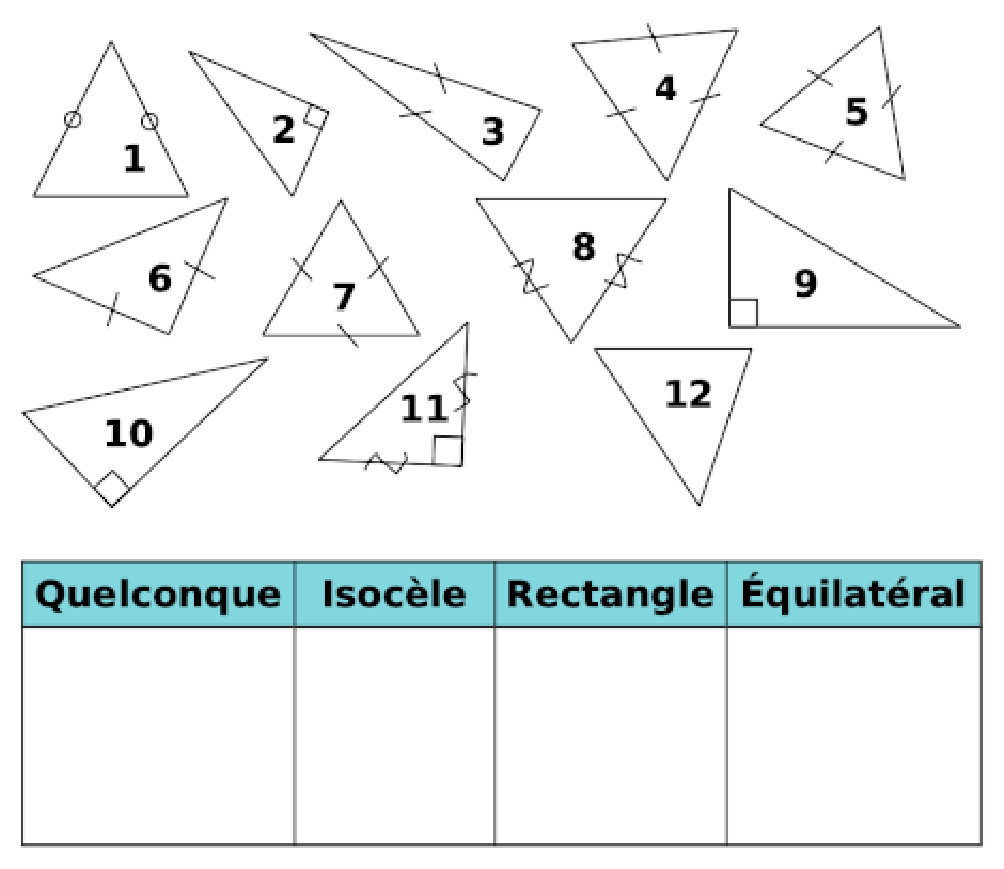
\includegraphics[width=8cm]{classement}
   \end{center}
\end{exercice}

\begin{exercice}
   On considère la figure suivante :
   \begin{center}
     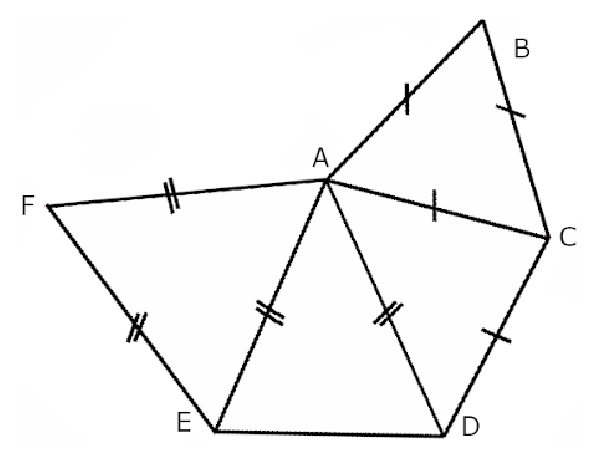
\includegraphics[width=4cm]{triangles}
   \end{center}
   \begin{enumerate}
      \item Nommer les triangles isocèles. Préciser, pour chacun, son sommet principal et sa base.
      \item Nommer les triangles équilatéraux tracés.
      \item Nommer les triangles isocèles que l'on peut tracer en joignant des sommets de la figure.
   \end{enumerate}
\end{exercice}

\serie{Construire des triangles} %%%%%%%%%%%

\begin{exercice}
   Un segment $[AB]$ mesure 7 cm. Construire sur la même figure, lorsque cela est possible, des points $M, N, P, Q$ et $R$ du même côté de $(AB)$, vérifiant les conditions ci-dessous.
   \begin{enumerate}
      \item $AM = 6$ cm et $BM = 4,5$ cm.
      \item $AN=4,8$ cm et $BN=2,2$ cm.
      \item $AP = 5$ cm et $BP = 12$ cm.
      \item $AQ=3,1$ cm et $BQ=3$ cm.
      \item $AR=11$ cm et $BR=4$ cm.
   \end{enumerate}
\end{exercice}

\begin{exercice}
   Tracer chacun des triangles suivants :
   \begin{enumerate}
      \item Le triangle $ABC$ tel que $AB =7$ cm ; $BC = 5$ cm et $CA =$ 6 cm.
      \item Le triangle $GHI$ tel que $HI = 5,1$ cm ; $GI = 5,6$ cm et $GH = 6,3$ cm.
      \item Le triangle équilatéral $EQU$ de périmètre 9 cm.
      \item Le triangle $RST$ isocèle en $S$ de périmètre 13 cm et tel que $ST=4$ cm.
      \item Le triangle $WHY$ rectangle en $W$ tel que \\ $WH =2,5$ cm et $WY =4$ cm.
   \end{enumerate}
\end{exercice}

\medskip

\begin{exercice}
   Voici les trois étapes de construction d'une figure.
   \begin{center}
      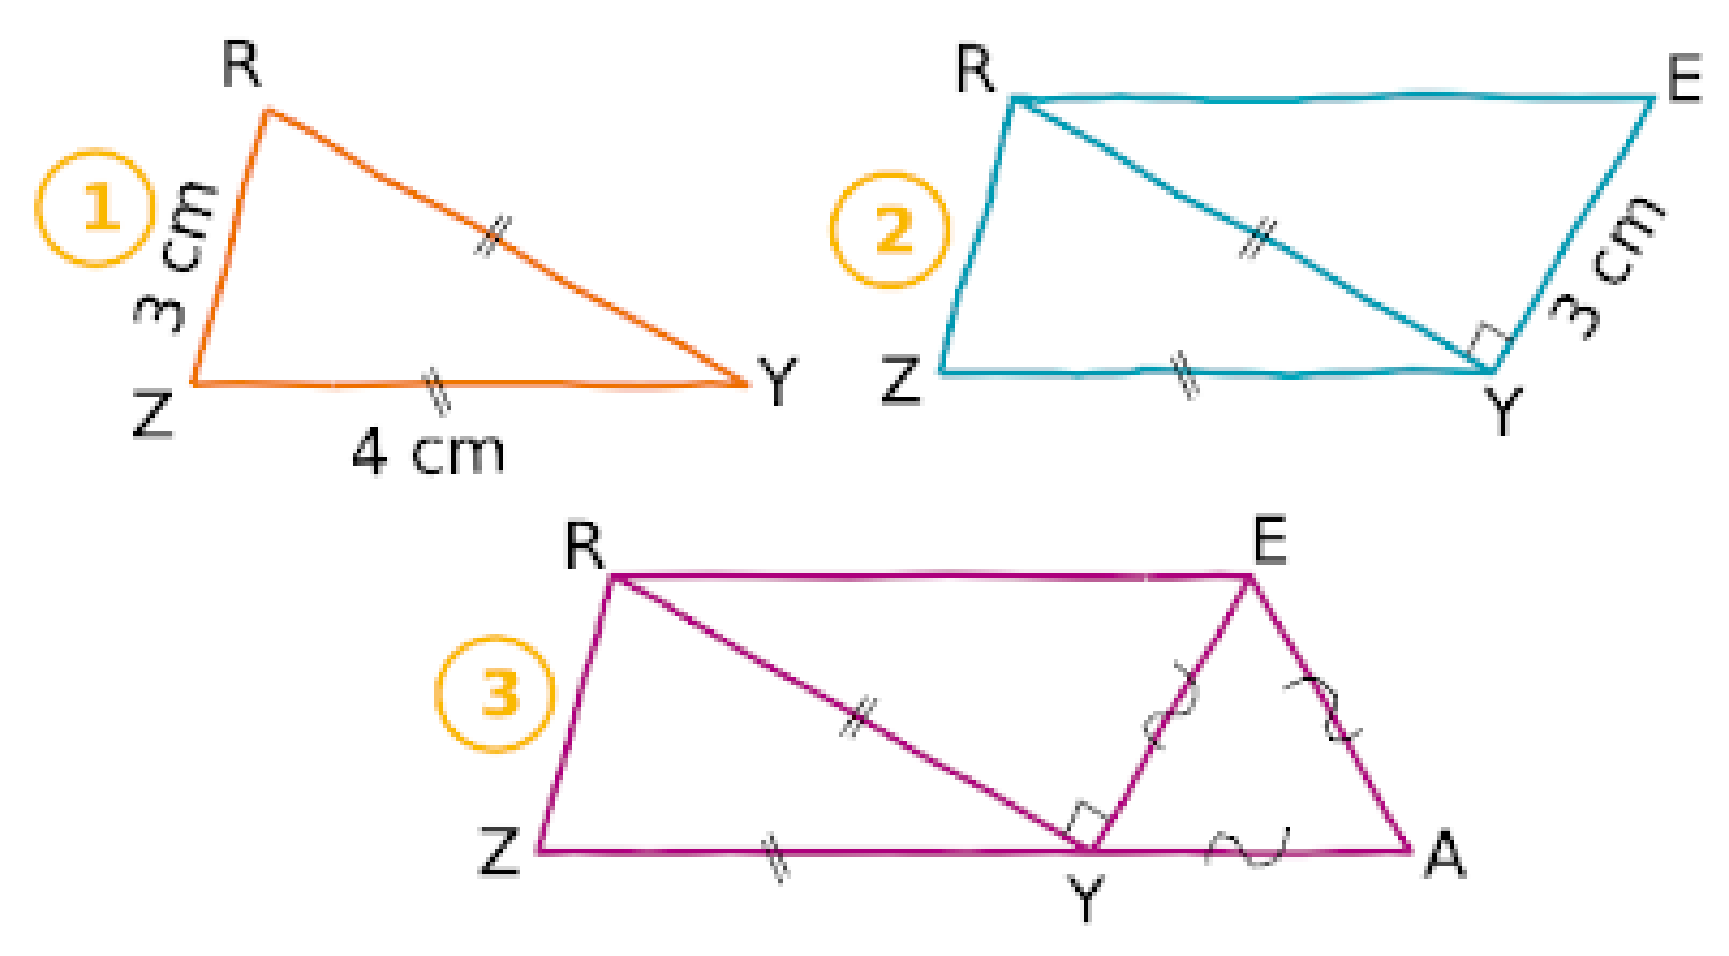
\includegraphics[width=7cm]{programme}
   \end{center}
   \vspace*{-6mm}
   \begin{enumerate}
      \item Écrire un programme permettant de construire la figure.
      \item Construire cette figure taille réelle.
   \end{enumerate}
\end{exercice}

\begin{exercice}
   Remettre les consignes du programme de construction dans l'ordre.
   \begin{center}
      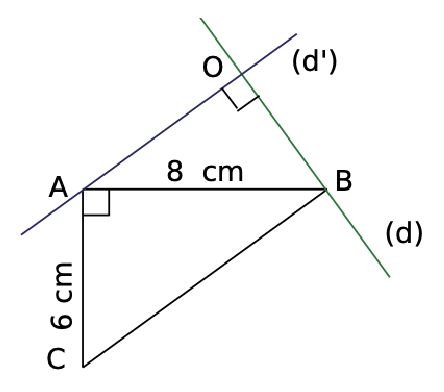
\includegraphics[width=4cm]{consignes}
   \end{center}
   \vspace*{-5mm}
   \begin{itemize}
      \item Trace la droite $(d')$ parallèle à la droite $(BC)$ passant par le point A.
      \item Nomme $O$ le point d'intersection des droites $(d)$ et $(d')$.
      \item Trace un triangle $ABC$ rectangle en $A$ tel que : \\
       $AB = 8$ cm et $AC = 6$ cm.
      \item Trace la droite $(d)$ perpendiculaire à la droite $(d')$ passant par $B$.
   \end{itemize}
\end{exercice}

\hfill {\it\footnotesize Source : Sesamath, le manuel 6\up{e}. Génération 5 - 2013}

\end{colonne*exercice}


%%%%%%%%%%%%%%%%%%%%%%%%%%%%%%%%%%%%%
%%%%%%%%%%%%%%%%%%%%%%%%%%%%%%%%%%%%%
\Recreation

   \enigme[Le triangle de Sierpinski]
     
   \partie[tracé du triangle]
       \begin{enumerate}
          \item Étape 1. Sur une feuille unie, tracer un triangle équilatéral de 16 cm de côté.
          \item Étape 2. 
          \begin{enumerate}
             \item Placer le milieu de chacun des trois côtés du triangle.
             \item Tracer le triangle équilatéral passant par les milieux des trois côtés à l'intérieur du grand triangle.
         \end{enumerate}
         \item Étape 3.
         \begin{enumerate}
            \item Pour les trois triangles situés aux sommets du triangle principal, placer les milieux des côtés.
            \item Construire les trois triangles à l'intérieur.
         \end{enumerate}
         \item Étape 4. Reproduire l'étape 3 pour chacun des neuf triangles ainsi construits.
         \item Décorer/colorier les triangles à votre guise.
     \end{enumerate}
     
      \begin{pspicture}(0.5,0)(4.5,4)
         \pspolygon(0,0)(4,0)(2,3.46)
      \end{pspicture}
      \multido{\i=1+1}{3}
         {\begin{pspicture}(4.5,4)
             \psSier(0,0){4cm}{\i}
          \end{pspicture}} \\
      \hspace*{0.9cm} Étape 1 \hspace*{3.3cm} Étape 2 \hspace*{3.3cm} Étape 3 \hspace*{3.3cm} Étape 4 \\
      
  \partie[dénombrement]
    \begin{enumerate}
       \item En se référant aux dessins ci-dessus, combien y a-t-il de triangles coloriés en noir à chaque étape ? \\ [2mm]
         Étape 1 : \dotfill Étape 2 : \dotfill Étape 3 : \dotfill Étape 4 : \dotfill \medskip
      \item Combien y aurait-il de triangles coloriés en noir à l'étape 5 ? \dotfill À l'étape 6 ? \dotfill
    \end{enumerate}
    
      \vfill

      \begin{center}
         \fbox{
            \begin{minipage}{13cm}
               {\bf Wacław Franciszek Sierpiński} (1882-1969) est un mathématicien polonais. \\
               Il s'intéresse entre autre aux fractales (une fractale est une forme géométrique qui se répète à l'identique lorsqu'on zoome ou qu'on \og dezoome\fg) dont certaines portent son nom : le triangle de Sierpiński, le tapis de Sierpiński et la courbe de Sierpiński. \\
               \begin{pspicture}(-0.7,0)(3,3.5)
                  \psSier(0,0){3cm}{5}
               \end{pspicture}
               \qquad
               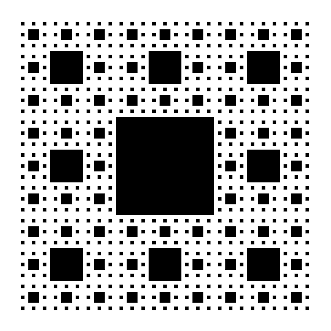
\includegraphics[width=3cm]{Sierpinski_carpet}
               \quad
               \begin{pspicture}(-2,-1.5)(2,1.5)
                  \psSier[unit=0.1,n=4,fillstyle=solid,fillcolor=black] 
               \end{pspicture}
               \medskip
            \end{minipage}}
      \end{center}


